\documentclass[tikz,border=10pt]{standalone}
% Scale s = 0.017621 cm/px (longest side = 8 cm), origin at O, y flipped
\begin{document}
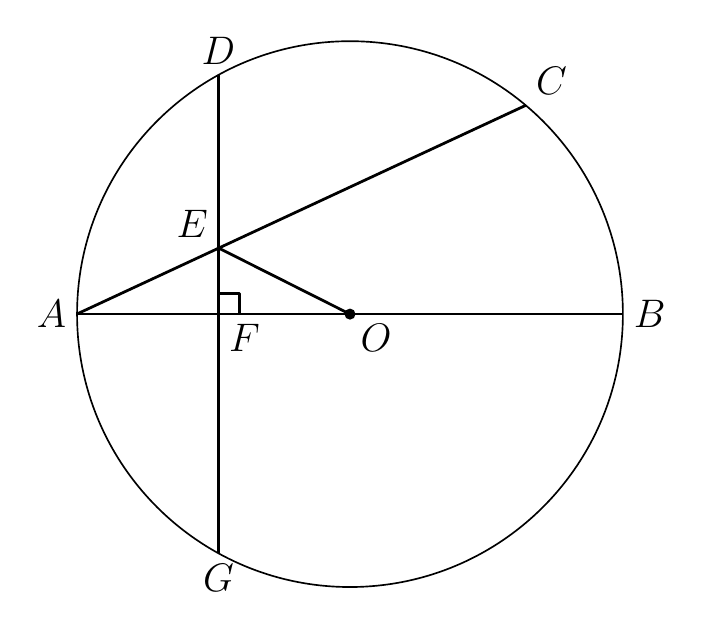
\begin{tikzpicture}[line join=round, line width=1.0pt]
  % Named coordinates (converted from pixels)
  \coordinate (O) at (0,0);
  \coordinate (A) at (-3.47,0.00);
  \coordinate (B) at (3.47,0.00);
  \coordinate (C) at (2.23,2.65);
  \coordinate (D) at (-1.67,3.04);
  \coordinate (E) at (-1.67,0.84);
  \coordinate (F) at (-1.67,0.00);
  \coordinate (G) at (-1.67,-3.04);

  % Circle (thin)
  \draw[line width=0.6pt] (O) circle (3.466);

  % Segments
  \draw (A) -- (B);
  \draw (D) -- (G);
  \draw (A) -- (C);
  \draw (O) -- (E);
  \draw (E) -- (F);

  % Right-angle marker at F (arms toward B and E)
  \draw (F) ++(0.264,0) -- ++(0,0.264) -- ++(-0.264,0);

  % Centre dot
  \fill (O) circle (2pt);

  % Labels
  \node[font=\fontsize{14.5}{17.4}\selectfont, left] at (A) {$A$};
  \node[font=\fontsize{14.5}{17.4}\selectfont, right] at (B) {$B$};
  \node[font=\fontsize{14.5}{17.4}\selectfont, above right] at (C) {$C$};
  \node[font=\fontsize{14.5}{17.4}\selectfont, above] at (D) {$D$};
  \node[font=\fontsize{14.5}{17.4}\selectfont, above left] at (E) {$E$};
  \node[font=\fontsize{14.5}{17.4}\selectfont, below right] at (F) {$F$};
  \node[font=\fontsize{14.5}{17.4}\selectfont, below] at (G) {$G$};
  \node[font=\fontsize{14.5}{17.4}\selectfont, below right] at (O) {$O$};
\end{tikzpicture}
\end{document}